\section{Repeated Measured Mitigation Comparison}\label{sec:measured-ab}
% Generated from complete measured mitigation campaign.
\newcommand{\MitigationRows}{
fixed/off & 1.000 [0.500, 1.601] & 0.506 [0.484, 0.526] & 0.720 [0.623, 0.816] \\
fixed/on & 0.050 [0.000, 0.150] & 0.493 [0.468, 0.519] & 0.667 [0.569, 0.763] \\
graded/off & 1.100 [0.600, 1.700] & 0.000 [0.000, 0.000] & 0.608 [0.512, 0.710] \\
graded/on & 0.100 [0.000, 0.250] & 0.000 [0.000, 0.000] & 0.713 [0.606, 0.821] \\
}

This experiment comprises 80 completed network trials: twenty independent seeds, each with fixed/graded policy
and guard off/on. Each seed reuses topology and workload parameters across arms and randomizes arm order. A fresh POX
process and Mininet network separate trials. The topology has 4--6 switches, two servers and three traffic sources.
This is an enforcement A/B experiment, \emph{not} the large-source capture experiment.

The falsely suspected source sends legitimate traffic to two destinations. We count its other-destination packets
lost during relative seconds $[1,3.25)$ as collateral, separately from loss for an unrelated legitimate source.
The attacker changes UDP source tuples to exercise learning and sends throughout three repeated block decisions.
Fixed policy converts the same suspicion request to a whole-host block; graded policy retains per-path suspicion
and requests increasing host TTLs. All results therefore compare identical evidence but intentionally different
response strength.

\begin{table*}[!tbp]
\caption{Actual WSL/Mininet enforcement: per-seed means and 95\% seed-bootstrap intervals}
\centering\footnotesize
\begin{tabular}{@{}llll@{}}
\toprule Policy / guard & Installation-window receipts & Collateral fraction & Suspicion to initial ACK (s) \\
\midrule
\MitigationRows
\bottomrule
\end{tabular}
\label{tab:measured-mitigation}
\end{table*}

\begin{figure*}[!tbp]
\centering
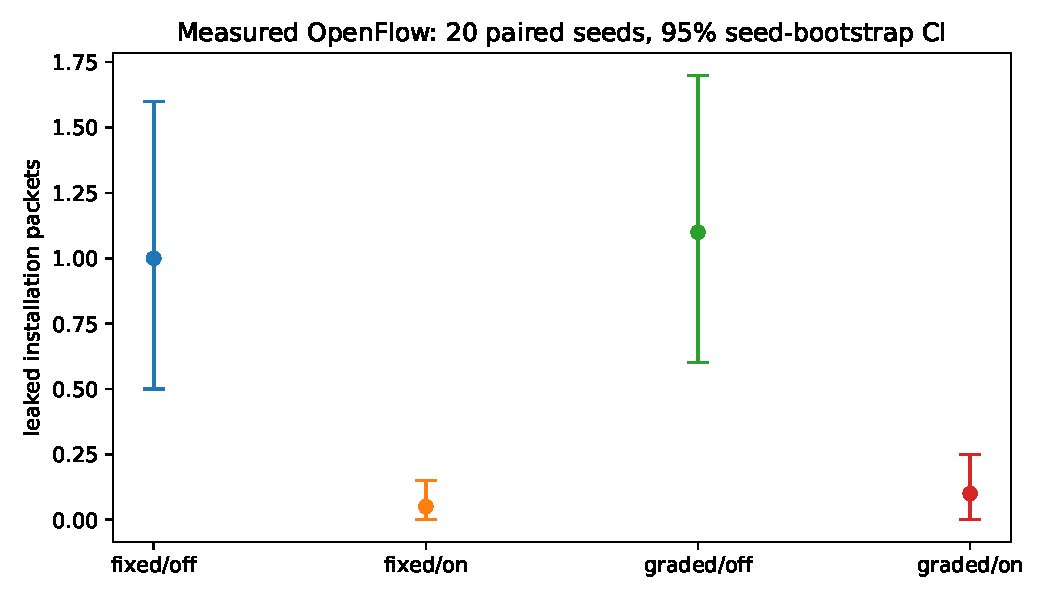
\includegraphics[width=.48\textwidth]{../results/mitigation_analysis_v3/15_leaked_installation_packets.pdf}
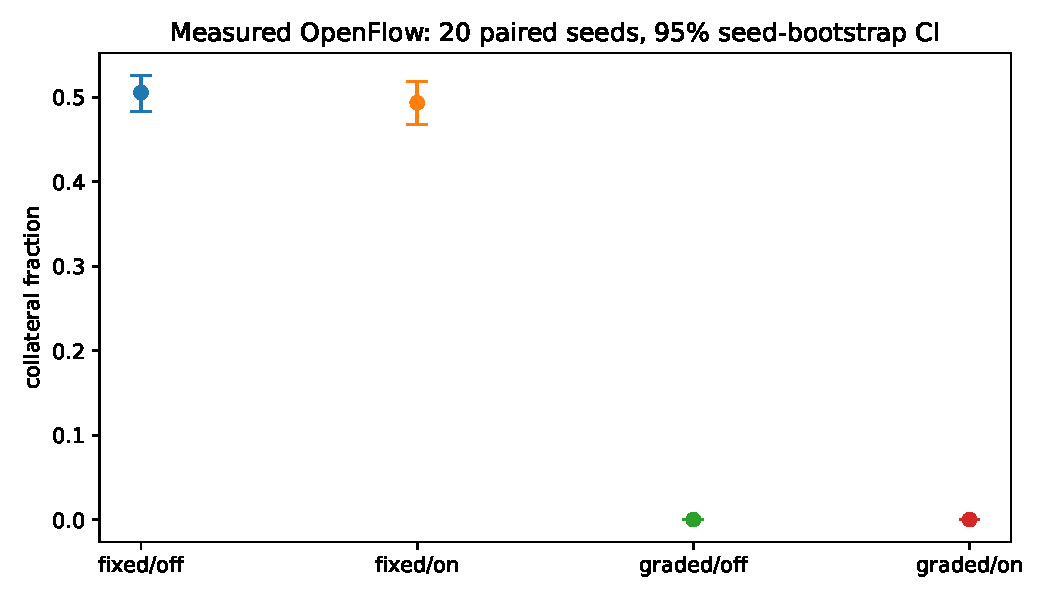
\includegraphics[width=.48\textwidth]{../results/mitigation_analysis_v3/16_collateral_fraction.pdf}\\
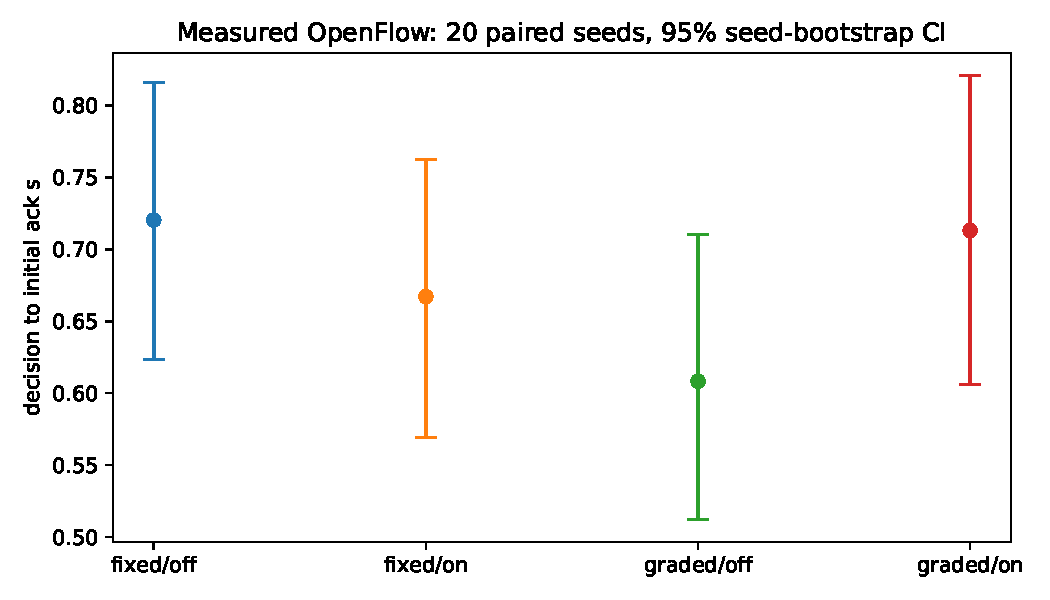
\includegraphics[width=.48\textwidth]{../results/mitigation_analysis_v3/17_decision_to_initial_ack_s.pdf}
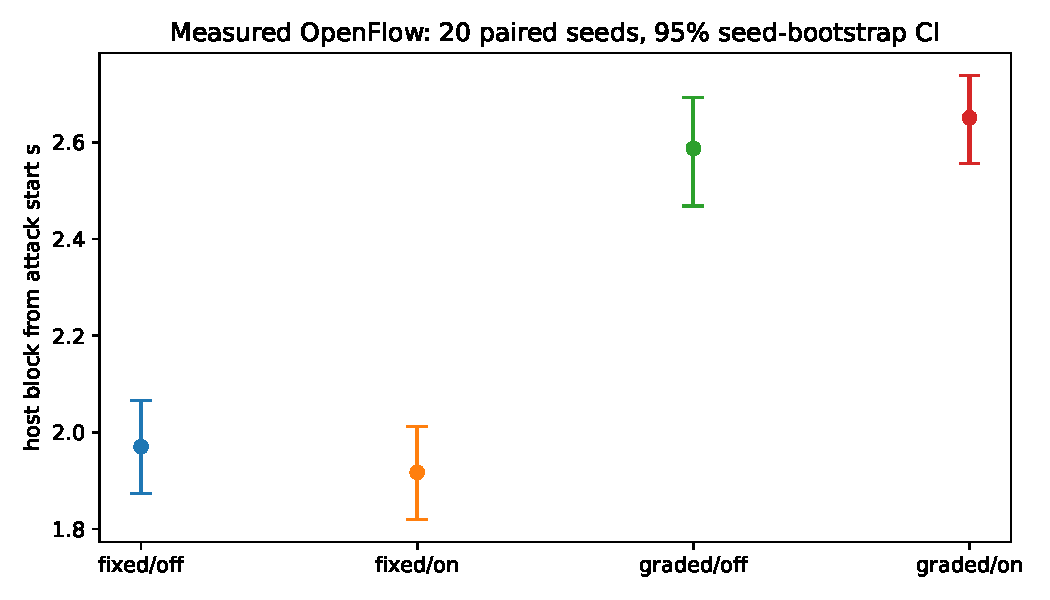
\includegraphics[width=.48\textwidth]{../results/mitigation_analysis_v3/18_host_block_from_attack_start_s.pdf}
\caption{Measured installation-window attacker receipts, benign collateral after injected false suspicion,
initial containment ACK time and full-host block ACK time. The interval ends at the last initial per-switch barrier
reply; packets already in flight are included, so these measurements do not identify the PacketIn race alone.}
\label{fig:measured-ab}
\end{figure*}

\begin{figure}[!tbp]
\centering
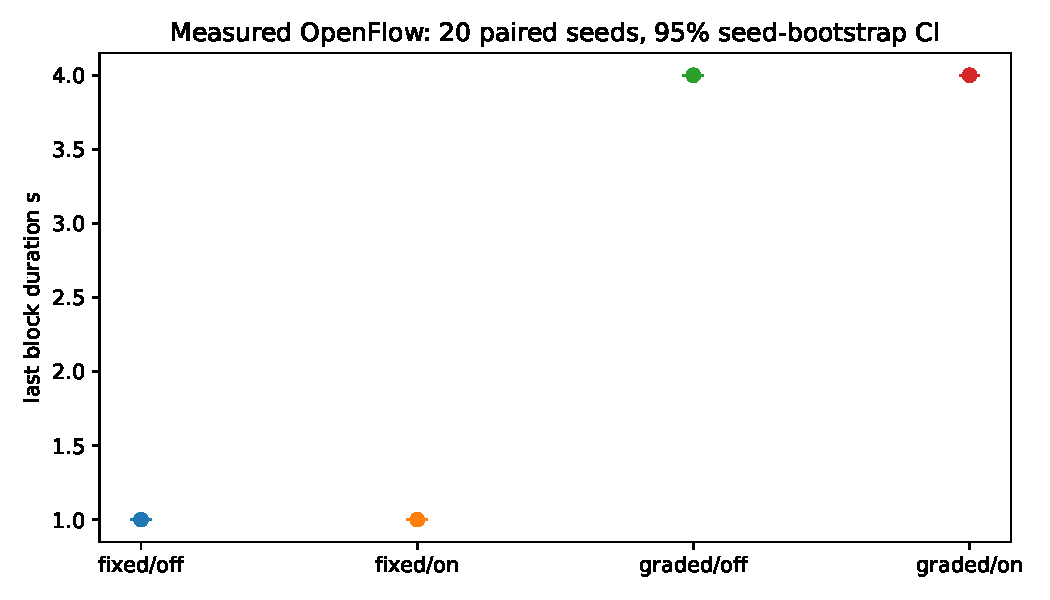
\includegraphics[width=\columnwidth]{../results/mitigation_analysis_v3/19_last_block_duration_s.pdf}
\caption{Accepted TTL on the final repeated host-block decision. Graded back-off increases the requested
duration; this is not by itself a measurement of victim availability or adaptive-attacker utility.}
\label{fig:measured-persistence}
\end{figure}

\begin{figure}[!tbp]
\centering
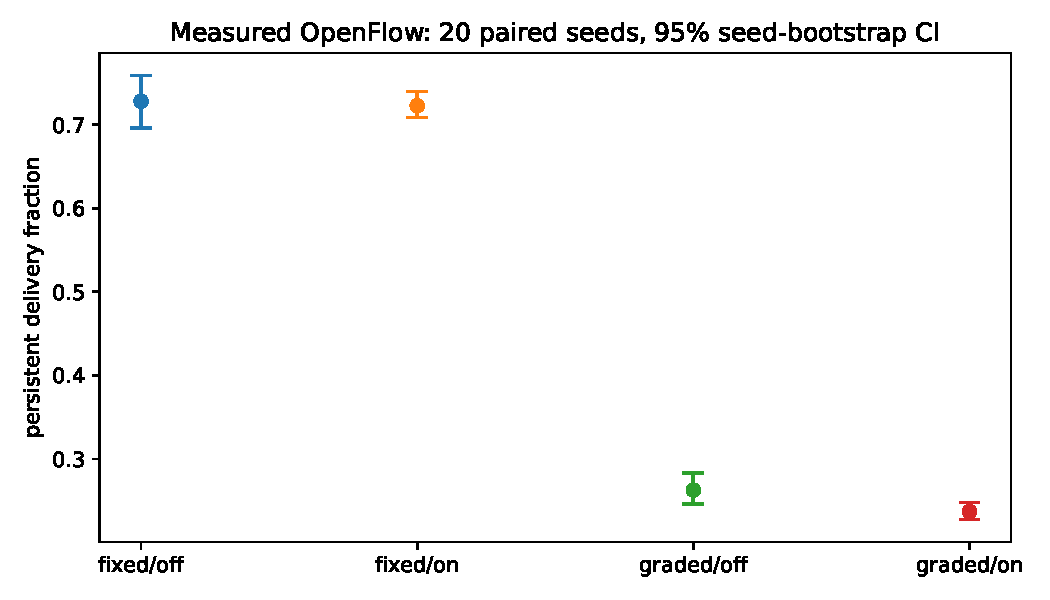
\includegraphics[width=\columnwidth]{../results/mitigation_analysis_v3/20_persistent_delivery_fraction.pdf}
\caption{Actual attacker delivery fraction from the second repeated decision to the end of traffic.
Sequence IDs join sent packets to receiver logs; longer accepted block TTL is not used as a substitute for this metric.}
\label{fig:measured-delivery}
\end{figure}

Paired effect intervals are provided in the artifact. A confidence interval containing zero is inconclusive,
not evidence that the guard improves leakage. Receiver timestamps measure actual arrivals, while barriers establish
installation ordering, not deletion of already queued packets. Short block durations, one-second decision polling,
WSL scheduling and synchronous trace I/O limit generalization. These measurements do not establish line-rate
capacity or a zero-leakage guarantee.
